\documentclass{article}
\usepackage[utf8]{inputenc}
\usepackage[spanish]{babel}
\usepackage{natbib}
\usepackage{graphicx}
\usepackage{mathtools}
\usepackage{color}
\usepackage{float}
\usepackage{fancyhdr}
\usepackage{adjustbox}


\pagestyle{fancy}
\lhead{Grupo 4 - Turno 7}
\chead{Trabajo Practico Nro 2}
\rhead{Primer Cuatrimestre 2015}

\begin{document}

\section{Objetivos}
	El objetivo del siguiente trabajo practico es determinar el vector campo eléctrico debido a la
aplicación de una diferencia de potencial entre dos zonas del espacio (electrodos). Para ello se
determinarán experimentalmente valores de diferencia de potencial en una grilla de puntos y
luego se calculará el campo eléctrico (módulo y dirección). También se tomarán líneas
equipotenciales con las que se podrá inferir la dirección del campo.

\section{Materiales}
	Para la experiencia se utilizaron los siguientes materiales:
    \begin{itemize}
		\item Cuba
        \item Electrodos
        \item Fuente
        \item Voltímetro
        \item Hojas milimetradas
	\end{itemize}

\section{Desarrollo}
\subsection{Procedimiento}
 En un recipiente plástico y cuasi-plano (que llamaremos cuba) con dos chapas metálicas lo más firmes posibles, las cuales funcionarán como nuestros electrodos, nos dispusimos a realizar el trabajo. Colocados los electrodos en dos esquinas de la diagonal de la cuba, conectamos a ellas una diferencia de potencial constante de 12V (que provee una fuente externa). En el borne negro de la fuente colocamos el terminal negro del voltímetro recibido, y con el terminal rojo, vamos midiendo el potencial de toda la grilla previamente dibujada en la hoja milimetrada.

Se midió:
    \begin{itemize}
		\item La grilla completa
        \item 12 puntos arbitrarios (4 en los bordes, 4 en el centro, 4 a elección)
        \item Las líneas de potencial 2V, 4V, 6V, 8V y 10V
        \item Los puntos alrededor de una lata sumergida en la cuba
	\end{itemize}

 
 Todas las mediciones se encuentran en la hoja de datos adjunta al trabajo.

\subsection{Preguntas}
	\begin{enumerate}
    	\item \textbf{¿ Las líneas de campo se pueden cortar entre sí? ¿Por qué?}
        
        No, porque las líneas de campo marcan la dirección del campo eléctrico. La recta 
        tangente en cada punto de la recta es igual a la dirección del campo eléctrico en ese 
        punto. Entonces si se cruzaran, el campo tendría mas de una dirección para el punto de 
        intersección y esto es imposible.
        
        \item \textbf{¿ En el segundo método, cuántos puntos son necesarios y/o adecuados 
        para determinarlos?}
        
        Esto es relativo, ya que lo que se hace es buscar una línea donde la diferencia de 
        potencial sea la misma y se desconoce su forma.
        
        \item \textbf{¿ Por qué no se puede establecer a priori el número de puntos que se 
        debe medir? }
        
        Como se dijo anteriormente, no se puede establecer un número determinado
        de puntos porque se desconoce la forma de las líneas equipotenciales, ya que esto
        depende de varios factores como por ejemplo, la forma de los electrodos.
        
        \item \textbf{¿ Por qué se usa agua en esta experiencia? ¿ Se podría medir la 
        diferencia de potencial en el aire? Sería mejor o peor usar agua destilada?}
        
        Se usa agua porque es necesario que circule corriente entre los electrodos para poder 
        medir la diferencia de potencial en los puntos intermedios. No se podría medir 
        directamente en el aire puesto que por este no circula corriente eléctrica. Sería 
        inútil usar agua destilada para la experiencia, ya que lo que permite que haya 
        corriente eléctrica son las sales disueltas en agua corriente (iones).
        
        \item \textbf{Vieron que la distribuciones de carga crean campos eléctricos.¿ Qué es 
        lo que produce el campo eléctrico que se quiere determinar en este caso?}
        
        Lo que genera el campo eléctrico en la experiencia son los 2 electrodos que están 
        conectados a la fuente con una diferencia de potencial constante.

        \item \textbf{El modelo más simple y útil para describir una corriente es que son 
        cargas en movimiento. En la experiencia el voltímetro mide una corriente.¿ Se puede 
        hablar, entonces, de campo electrostático?}
        
        Al producirse movimiento de cargas no se puede hablar de campo electrostático, pero 
        como es conservativo se puede analizar de la misma forma. 

	\end{enumerate}

\section{Hoja de datos}
El objetivo de la hoja milimetrada adjunta, es poder observar gráficamente los datos obtenidos durante la experiencia y establecer relaciones claras y de forma rápida.\\
En primer lugar, encontramos que la hoja está marcada con líneas cada dos centímetros, formando una cierta cantidad de puntos de intersección. Además, en color celeste, encontramos la representación de los electrodos utilizados, indicando su polaridad.
En todos los puntos de intersección (de aquí en adelante, vértices) donde es viable medir utilizando el téster, obtuvimos un valor de potencial sobre la totalidad de la grilla.\\
A continuación, elegimos doce vértices (cuatro en el centro, cuatro en el borde y cuatro a elección) para los cuáles realizaremos una segunda medición de su potencial; estos valores estarán subrayados en color violeta para identificarlos rápidamente con la vista.\\
Una vez realizadas estas mediciones, procedemos a introducir una lata metálica (diámetro 7,6cm y altura 9,4cm) en la cuba. Luego, realizamos una tercera medición con el objetivo de observar cómo varía el potencial cuando introducimos un conductor en la cuba. Estas mediciones se encuentran recuadradas con color rosa.\\
Todos los puntos que tengan un número redondeado (2,4,6,8 o 10) son los puntos por dónde pasa la línea equipotencial de ese valor. En consecuencia, el trazado de las líneas de campo se hará de forma tal que pasen por esos puntos; las líneas de campo se encuentran dibujadas en la hoja de calcar que se encuentra adjunta a la hoja de datos. Por colores, distinguimos a que valor corresponde cada una: naranja -> potencial 2V,azul -> potencial 4V, verde -> potencial 6V, marrón -> potencial 8V, rojo -> potencial 10V.\\
La segunda hoja milimetrada, tiene los doce puntos mencionados anteriormente y, cada uno de ellos, tiene su campo eléctrico (módulo y componentes) graficado.

\section{Resultados}
	\subsection{Experimentales}
		\begin{table}[H]
        \begin{adjustbox}{max width=\columnwidth}
        	%%%%%%%%%%%%%%%%%%%%%%%%%%%%%%%%%%%%%%%%%%%%%%%%%%%%%%%%%%%%%%%%%%%%%%
%%                                                                  %%
%%  This is a LaTeX2e table fragment exported from Gnumeric.        %%
%%                                                                  %%
%%%%%%%%%%%%%%%%%%%%%%%%%%%%%%%%%%%%%%%%%%%%%%%%%%%%%%%%%%%%%%%%%%%%%%
\begin{tabular}{| c | c | c | c |}
\hline
 & \multicolumn{3}{|c|}{Voltaje (V)} \\ \cline{2-4}
Distancia (mm)	& $1^a$ Medición	&$2^a$ Medición	& $3^a$ Medición\\ \hline
3	&4.4	&4.4	&3.8\\
4	&4.8	&4.8	& 4.2\\
5	&5.3	&5	    &4.4\\
6	&5.6	&5.3	&4.6\\
7	&6	    &5.6	&4.8\\
8	&6.2	&5.8	&5\\
9	&6.4	&6	    &5.1\\
10	&6.4	&6	    &5.2\\
11	&6.6	&6.1	&5.2\\
12	&6.8	&6.2	&5.4\\
13	&6.8	&6.3	&5.6\\
14	&6.8	&6.4	&5.6\\
15	&6.8	&6.4	&5.6\\
16	&6.9	&6.4	&5.6\\
17	&7.2	&6.4	&5.6\\
18	&7.2	&6.5	&5.6\\
19	&7.2	&6.6	&5.7\\
20	&x	    &x	    &5.7\\
25	&x	    &x	    &5.9\\
30	&7.4	&6.8	&6\\
35	&x	    &6.8	&6\\
40	&x	    &x	    &6\\
45	&x	    &x	    &6\\
50	&x	    &x	    &6\\ \hline
\end{tabular}
        \end{adjustbox}
        \caption{Mediciones de potencial (V)}
        \end{table}
    	\begin{table}[H]
        \begin{adjustbox}{max width=\columnwidth}
        	%%%%%%%%%%%%%%%%%%%%%%%%%%%%%%%%%%%%%%%%%%%%%%%%%%%%%%%%%%%%%%%%%%%%%%
%%                                                                  %%
%%  This is a LaTeX2e table fragment exported from Gnumeric.        %%
%%                                                                  %%
%%%%%%%%%%%%%%%%%%%%%%%%%%%%%%%%%%%%%%%%%%%%%%%%%%%%%%%%%%%%%%%%%%%%%%
\begin{tabular}{| l || c | c | c | c | c | c | c | c | r |}
\hline
9   &5.67	&6.12	&6.64	&7.27	&8	    &8.9	&x	    &x	    &x\\
8   &5.41	&5.85	&6.38	&6.97	&7.6	&8.43	&9.52	&x	    &x\\
7   &5.06	&5.5	&6.06	&7.15	&7.74	&8.59	&9.47	&9.52	&x\\
6   &4.6	&5.08	&5.73	&x	    &x	    &x	    &x	    &9.47	&9.48\\
5   &4.4	&4.6	&5.45	&x	    &x	    &x	    &x	    &8.58	&8.71\\
4   &3.2	&3.9	&4.9	&x	    &x	    &x	    &x	    &7.95	&8.19\\
3   &x	    &3	    &4.15	&5.33	&x	    &x	    &6.83	&7.56	&7.77\\
2   &x	    &x	    &x	    &4.51	&5.33	&5.97	&6.5	&7	    &7.45\\
1   &x	    &x	    &x	    &3.9	&4.86	&5.62	&6.23	&x	    &x\\ \hline \hline
y/x &3	    &4	    &5	    &6	    &7	    &8	    &9	    &10	    &11\\ \hline
\end{tabular}
        \end{adjustbox}
        \caption{Mediciones de potencial con lata dentro de la cuba (V)}
        \end{table}
    
    \subsection{Analíticos}
    Los cálculos del campo eléctrico fueron hechos a partir de las resultados experimentales de la cuba sin la presencia de la lata.
		\begin{table}[H]
        \begin{adjustbox}{max width=\columnwidth}
        	%%%%%%%%%%%%%%%%%%%%%%%%%%%%%%%%%%%%%%%%%%%%%%%%%%%%%%%%%%%%%%%%%%%%%%
%%                                                                  %%
%%  This is a LaTeX2e table fragment exported from Gnumeric.        %%
%%                                                                  %%
%%%%%%%%%%%%%%%%%%%%%%%%%%%%%%%%%%%%%%%%%%%%%%%%%%%%%%%%%%%%%%%%%%%%%%
\begin{tabular}{| l || c | c | c | c | c | c | c | c | c | c | c | c | c | r |}
\hline
9   &0.0975	&0.1525	&0.205	&0.2675	&0.33	&0.38	&0.4475	&-1.975	&-6.905	&x	    &x	    &x	    &x	    &x\\
8   &0.4625	&0.2775	&0.21	&0.2675	&0.33	&0.35	&0.425	&0.5175	&0.4825	&0.3975	&x	    &x	    &x	    &x\\
7   &0.085	&0.155	&0.2175	&0.28	&0.3175	&0.3625	&0.1625	&0.42	&0.6675	&0.375	&0.2825	&0.1775	&x	    &x\\
6   &0.04	&0.15	&0.23	&0.285	&0.3425	&0.375	&0.375	&0.3775	&0.375	&0.3325	&0.2575	&0.1625	&0.0575	&x\\
5   &0.085	&0.165	&0.2325	&0.3075	&0.35	&0.37	&0.39	&0.3625	&0.3325	&0.2925	&0.235	&0.1725	&0.1	&0.03\\
4   &0.045	&0.175	&0.295	&0.3525	&0.3775	&0.415	&0.4	&0.3625	&0.325	&0.2725	&0.23	&0.1725	&0.11	&0.06\\
3   &x	    &x	    &0.3425	&0.4375	&0.4625	&0.44	&0.4125	&0.36	&0.3175	&0.2825	&0.2325	&0.17	&0.115	&0.065\\
2   &x	    &x	    &x	    &x	    &0.5675	&0.5125	&0.4375	&0.3675	&0.3225	&0.2725	&0.22	&0.1675	&0.115	&0.065\\
1   &x	    &x	    &x	    &x	    &x	    &0.5425	&0.4575	&0.4325	&0.325	&0.2225	&0.2175	&0.17	&0.1175	&0.0525\\ \hline \hline
y/x &1	    &2	    &3	    &4	    &5	    &6	    &7	    &8	    &9	    &10	    &11	    &12	    &13	    &14\\ \hline
\end{tabular}
        \end{adjustbox}
        \caption{Valores de $E_x \left(\frac{V}{m}\right)$}
        \end{table}
        
        \begin{table}[H]
        \begin{adjustbox}{max width=\columnwidth}
        	%%%%%%%%%%%%%%%%%%%%%%%%%%%%%%%%%%%%%%%%%%%%%%%%%%%%%%%%%%%%%%%%%%%%%%
%%                                                                  %%
%%  This is a LaTeX2e table fragment exported from Gnumeric.        %%
%%                                                                  %%
%%%%%%%%%%%%%%%%%%%%%%%%%%%%%%%%%%%%%%%%%%%%%%%%%%%%%%%%%%%%%%%%%%%%%%
\begin{tabular}{| l || c | c | c | c | c | c | c | c | c | c | c | c | c | r |}
\hline
9   &0.64	&0.1475	&0.1425	&0.14	&0.155	&0.1275	&0.2575	&-0.067	&-7.317	&x	    &x	    &x	    &x	    &x\\
8   &-0.195	&0.1925	&0.1875	&0.18	&0.175	&0.1925	&0.1925	&0.4775	&-2.203	&0.3725	&x	    &x	    &x	    &x\\
7   &0.255	&0.2625	&0.2525	&0.2425	&0.235	&0.23	&0.21	&0.28	&0.35	&0.4175	&0.45	&0.47	&x	    &x\\
6   &0.285	&0.3125	&0.305	&0.2975	&0.2775	&0.265	&0.27	&0.0375	&0.3275	&0.3725	&0.41	&0.42	&0.4025	&x\\
5   &0.375	&0.3975	&0.38	&0.3325	&0.3125	&0.2975	&0.2725	&0.2725	&0.2875	&0.3225	&0.3475	&0.35	&0.3375	&0.3\\
4   &0.525	&0.5625	&0.4675	&0.4025	&0.3375	&0.29	&0.2675	&0.2675	&0.27	&0.2825	&0.28	&0.285	&0.2825	&0.2825\\
3   &x	    &x	    &0.5125	&0.4975	&0.3275	&0.2575	&0.23	&0.22	&0.225	&0.2225	&0.225	&0.2325	&0.23	&0.2225\\
2   &x	    &x	    &x	    &x	    &0.3425	&0.2175	&0.1875	&0.1725	&0.115	&0.165	&0.175	&0.18	&0.175	&0.1725\\
1   &x	    &x	    &x	    &x	    &x	    &0.1825	&0.1825	&0.1475	&-0.005	&0.145	&0.135	&0.14	&0.125	&0.1325\\ \hline \hline
y/x &1	    &2	    &3	    &4	    &5	    &6	    &7	    &8	    &9	    &10	    &11	    &12	    &13	    &14\\ \hline
\end{tabular}
        \end{adjustbox}
        \caption{Valores de $E_y \left(\frac{V}{m}\right)$}
        \end{table}
 
 		\begin{table}[H]
        \begin{adjustbox}{max width=\columnwidth}
        	%%%%%%%%%%%%%%%%%%%%%%%%%%%%%%%%%%%%%%%%%%%%%%%%%%%%%%%%%%%%%%%%%%%%%%
%%                                                                  %%
%%  This is a LaTeX2e table fragment exported from Gnumeric.        %%
%%                                                                  %%
%%%%%%%%%%%%%%%%%%%%%%%%%%%%%%%%%%%%%%%%%%%%%%%%%%%%%%%%%%%%%%%%%%%%%%
\begin{tabular}{| l || c | c | c | c | c | c | c | c | c | c | c | c | c | r |}
\hline
9   &0.647	&0.212	&0.250	&0.302	&0.365	&0.401	&0.516	&1.976	&10.061	&x	    &x	    &x	    &x	    &x\\
8   &0.502	&0.338	&0.282	&0.322	&0.374	&0.399	&0.467	&0.704	&2.255	&0.545	&x	    &x	    &x	    &x\\
7   &0.269	&0.305	&0.333	&0.370	&0.395	&0.429	&0.266	&0.505	&0.754	&0.561	&0.531	&0.502	&x	    &x\\
6   &0.288	&0.347	&0.382	&0.412	&0.441	&0.459	&0.462	&0.379	&0.498	&0.499	&0.484	&0.450	&0.407	&x\\
5   &0.385	&0.430	&0.445	&0.453	&0.469	&0.475	&0.476	&0.454	&0.440	&0.435	&0.420	&0.390	&0.352	&0.301\\
4   &0.527	&0.589	&0.553	&0.535	&0.506	&0.506	&0.481	&0.451	&0.423	&0.393	&0.362	&0.333	&0.303	&0.289\\
3   &x	    &x	    &0.616	&0.663	&0.567	&0.510	&0.472	&0.422	&0.389	&0.360	&0.324	&0.288	&0.257	&0.232\\
2   &x	    &x	    &x	    &x	    &0.663	&0.557	&0.476	&0.406	&0.342	&0.319	&0.281	&0.246	&0.209	&0.184\\
1   &x	    &x	    &x	    &x	    &x	    &0.572	&0.493	&0.457	&0.325	&0.266	&0.256	&0.220	&0.172	&0.143\\ \hline \hline
y/x &1	    &2	    &3	    &4	    &5	    &6	    &7	    &8	    &9	    &10	    &11	    &12	    &13	    &14\\ \hline
\end{tabular}
        \end{adjustbox}
        \caption{Valores del modulo de $E \left(\frac{V}{m}\right)$}
        \end{table}
        
        \subsection{Numéricos}
        Hemos utilizado el programa FEMM para recrear el experimento realizado en el laboratorio.\\
        
Comparamos nuestro resultados experimentales con las siguientes simulaciones:

\begin{figure}[H]
\centering
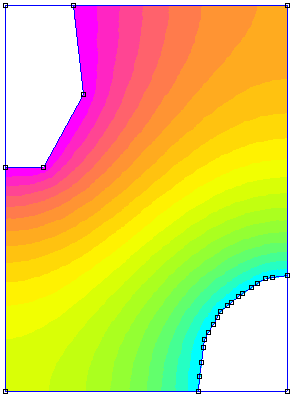
\includegraphics[scale=1]{cuba.png}
\caption{Simulación de cuba}
\label{fig:1}
\end{figure}  
        
\begin{figure}[H]
\centering
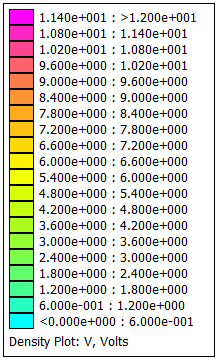
\includegraphics[scale=1]{escala.png}
\caption{Escala utilizada}
\label{fig:2}
\end{figure} 

Estos son los resultados obtenidos a partir de la simulación en femm.
        \begin{table}[H]
        \centering
        \begin{adjustbox}{max width=\columnwidth}
        	%%%%%%%%%%%%%%%%%%%%%%%%%%%%%%%%%%%%%%%%%%%%%%%%%%%%%%%%%%%%%%%%%%%%%%
%%                                                                  %%
%%  This is a LaTeX2e table fragment exported from Gnumeric.        %%
%%                                                                  %%
%%%%%%%%%%%%%%%%%%%%%%%%%%%%%%%%%%%%%%%%%%%%%%%%%%%%%%%%%%%%%%%%%%%%%%
\begin{tabular}{| l | c | r |}
\hline
X	&Y	&Potencial (V)\\ \hline
3 	&3 	&0.86\\
5 	&2	&2.86\\
4 	&5 	&4.23\\
7 	&3 	&5.87\\
5 	&6 	&6.03\\
7 	&5 	&7.20\\
6 	&7	&7.83\\
9 	&3	&7.53\\
7 	&6 	&8.03\\
9 	&5	&8.79\\
10 	&8	&11.40\\
12 	&7	&11.49\\ \hline
\end{tabular}
        \end{adjustbox}
        \caption{Potencial dentro de la cuba}
        \end{table}
        
\begin{figure}[H]
\centering
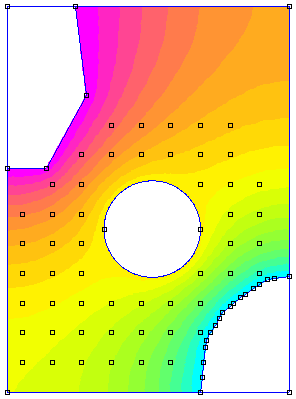
\includegraphics[scale=1]{cubaConLata.png}
\caption{Simulación de cuba con lata}
\label{fig:3}
\end{figure}  
        
        \begin{table}[H]
        \begin{adjustbox}{max width=\columnwidth}
%%%%%%%%%%%%%%%%%%%%%%%%%%%%%%%%%%%%%%%%%%%%%%%%%%%%%%%%%%%%%%%%%%%%%%
%%                                                                  %%
%%  This is a LaTeX2e table fragment exported from Gnumeric.        %%
%%                                                                  %%
%%%%%%%%%%%%%%%%%%%%%%%%%%%%%%%%%%%%%%%%%%%%%%%%%%%%%%%%%%%%%%%%%%%%%%
\begin{tabular}{| l || c | c | c | c | c | c | c | c | r |}
\hline
9   &5.48	&5.77	&6.25	&6.92	&7.83	&9.08	&x	    &x	    &x\\
8   &5.28	&5.59	&6.06	&5.88	&7.48	&8.58	&10.2	&x	    &x\\
7   &4.88	&5.23	&5.73	&6.32	&6.85	&7.57	&8.82	&10.23	&x\\
6   &4.25	&4.69	&5.37	&x	    &x	    &x	    &7.57	&8.78	&9.9\\
5   &3.31	&3.9	&4.9	&x	    &x	    &x	    &x	    &7.76	&8.84\\
4   &1.99	&2.68	&4	    &x	    &x	    &x	    &x	    &7.26	&8.14\\
3   &x	    &0.81	&2.33	&4.34	&x	    &x	    &6.33	&6.97	&7.67\\
2   &x	    &x	    &x	    &2.42	&4.15	&5.23	&6	    &6.69	&7.34\\
1   &x	    &x	    &x	    &0.94	&3.09	&4.58	&5.64	&x	    &x\\ \hline \hline
y/x &3	    &4	    &5	    &6	    &7	    &8	    &9	    &10	    &11\\ \hline
\end{tabular}
        \end{adjustbox}
        \caption{Potencial con lata dentro de la cuba}
        \end{table}      

\section{Discusiones y Conclusiones}
\begin{itemize}
		\item El sistema de trabajo, por su rusticidad, hace que sea muy difícil obtener una medición idéntica a otra en el mismo punto. La forma en que se apoya el téster, cuidando el paralaje, y su contacto con la superficie, el hecho de que el fondo de la cuba no sea perfectamente plano, entre otros, son factores que influyeron en las mediciones.
		\item Verificamos que el comportamiento de las líneas equipotenciales es el esperado y por lo tanto el de las líneas de campo también, las líneas equipotenciales nunca se cortaron entre si, estas van disminuyendo su potencial con la cercanía a el borne negativo y son perpendiculares a las líneas de campo.
        \item Comprobamos que el campo en cada punto, es perpendicular a la línea de campo a la que pertenece.
        \item Comprobamos con datos experimentales y el apoyo de la simulación, que las líneas de campo y las equipotenciales se modifican al introducir la lata conductora en la cuba. Esto se debe a que el campo eléctrico entra y sale en dirección perpendicular a la superficie de los conductores (electrodos y lata).
        \item Al configurar una simulación lo más cercana posible a la realidad, obtuvimos los resultados ideales para la experiencia realizada y observamos que el error entre los resultados experimentales e ideales es menor al 2\%.\\
Si bien no coinciden perfectamente, la razón se debe a que la cantidad de valores medidos en el laboratorio fueron mucho menores a los puntos donde el programa hizo sus cálculos, y a que en la medición manual y el procesamiento posterior hay más posibilidad de acumular errores.
       
	\end{itemize}.
\end{document}